\documentclass[a4paper,11pt]{article}
\usepackage{color}
\usepackage{graphicx}
\usepackage{subcaption}
\usepackage{amsmath}
\usepackage{tikz}
\usepackage{listings}
\definecolor{codegreen}{rgb}{0,0.6,0}
\definecolor{codegray}{rgb}{0.5,0.5,0.5}
\definecolor{codepurple}{rgb}{0.58,0,0.82}
\definecolor{backcolour}{rgb}{0.95,0.95,0.92}
 
\lstdefinestyle{mystyle}{
    backgroundcolor=\color{backcolour},   
    commentstyle=\color{codegreen},
    keywordstyle=\color{magenta},
    numberstyle=\tiny\color{codegray},
    stringstyle=\color{codepurple},
    basicstyle=\footnotesize,
    breakatwhitespace=false,         
    breaklines=true,                 
    captionpos=b,                    
    keepspaces=true,                 
    numbers=left,                    
    numbersep=5pt,                  
    showspaces=false,                
    showstringspaces=false,
    showtabs=false,                  
    tabsize=2
}
 
\lstset{style=mystyle}
\usetikzlibrary{automata,positioning}

\graphicspath{ {images/} }
\begin{document}
\title{\color{red}CARNEGIE MELLON UNIVERSITY\\
APPLIED STOCHASTIC PROCESSES  (COURSE 18-751)\\
HOMEWORK 8}
\author{Daniel Marew}
\date{\today}
\clearpage\maketitle

\thispagestyle{empty}
\newpage
I collaborated with :\\
\hspace*{6cm}
Nebyou Yismaw\\
\hspace*{6cm}
Daniel    Nkemelu\\
\hspace*{6cm}
Agatha Niwomugizi
\thispagestyle{empty}
\newpage
\clearpage
\setcounter{page}{1}
\section*{Q.1}
\subsection*{(a)}
\begin{figure}[h]
  \hspace*{-6cm}
   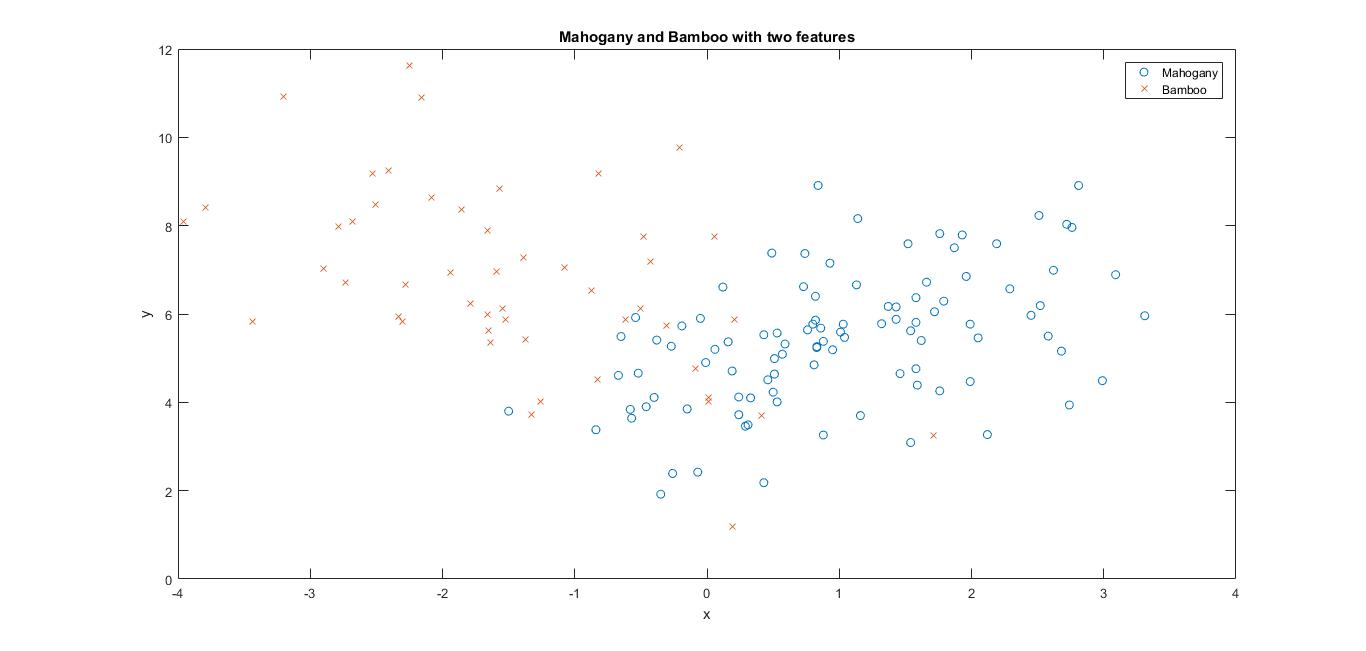
\includegraphics[scale=0.5]{q1_a}
   \caption{Mahogany and Bamboo with two features}\label{fig:q1_a}
\end{figure}
\subsection*{(b)}
$$P[M] = \frac{\#Number of Mahogany In Sample}{\#Total Sample Size} = \frac{100}{150}=\frac{2}{3}$$
$$P[B] = \frac{\#Number of Bamboo In Sample}{\#Total Sample Size} = \frac{50}{150}=\frac{1}{3}$$
$$\mu_{M_x} =\frac{1}{M} \sum_{x}^{}M_x = 1.0044$$
$$\mu_{M_y} =\frac{1}{M} \sum_{y}^{}M_y = 5.4160$$
$$\mu_M = [1.0044,5.4160]^T$$
$$\mu_{B_x} =\frac{1}{B} \sum_{x}^{}B_x = -1.4752$$
$$\mu_{B_y} =\frac{1}{B} \sum_{y}^{}B_y =  6.7724$$
$$\mu_B = [-1.4752,6.7724]^T$$

    \[
cov[X,Y]_M = K_M =
  \begin{bmatrix}
    1.0852 & 0.7399  \\
     0.7399 &2.1879 
  \end{bmatrix}
\]
    \[
cov[X,Y]_B = K_B =
  \begin{bmatrix}
    1.3980 & -1.3145  \\
     -1.3145 &4.4088
  \end{bmatrix}
\]
\newpage
\clearpage
\subsection*{(c) Linear Estimators}
$$\hat{Y}(x) = \mu_Y+\rho\frac{\sigma_Y}{\sigma_X}(x-\mu_X)$$
the slope is given by 
$$slope = \rho \frac{\sigma_Y}{\sigma_X}$$
and the Intercept 
$$Intercept = \mu_Y - \rho \frac{\sigma_Y}{\sigma_X}\mu_X$$
\begin{figure}[h]
  \hspace*{-6cm}
   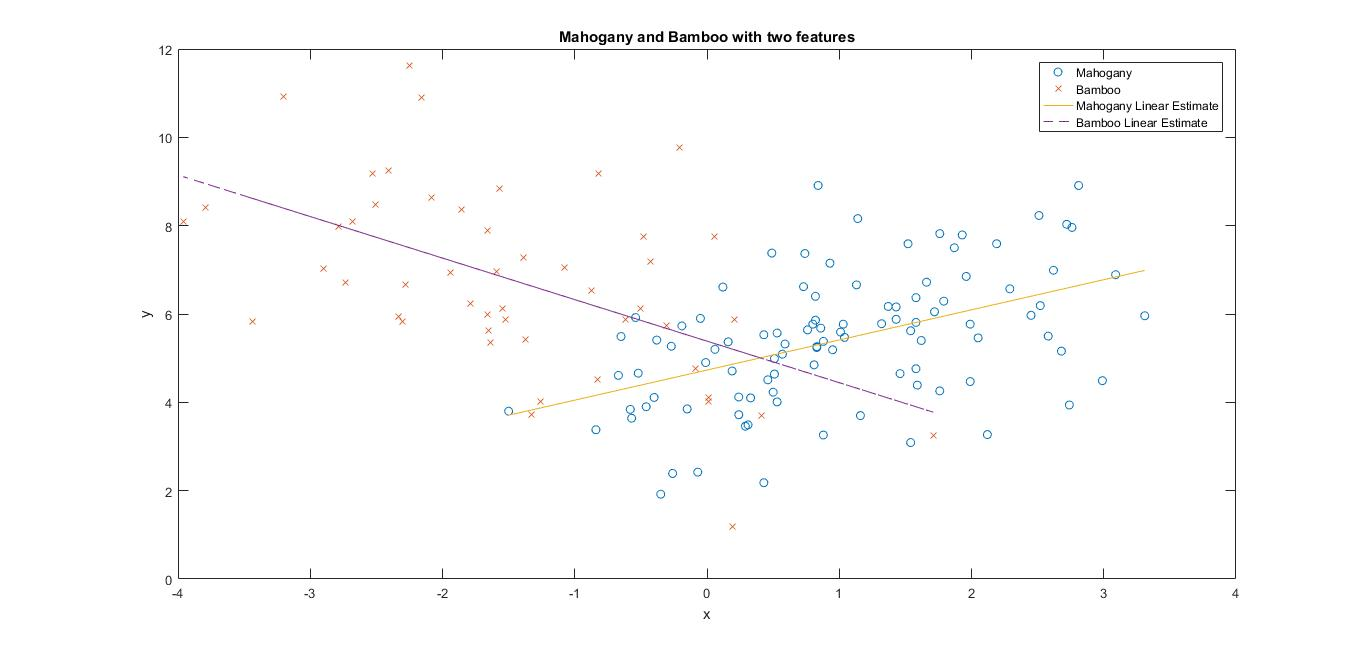
\includegraphics[scale=0.5]{q1_c}
   \caption{Mahogany and Bamboo with two features}\label{fig:q1_c}
\end{figure}
\clearpage
\newpage
\quad \\
Ans.\\
Using the equations above we get\\
Mahogany Linear Estimator Slope $=  0.68$\\
Mahogany Linear Estimato  Intercept=$4.73$ \\
Bamboo Linear Estimator Slope=$-0.94$\\ 
Bamboo Linear Estimator Intercept$=5.39$ \\
\subsection*{(d)}
$$a = K_W^{-1}(\mu_M-\mu_B)$$

 \[
K_W^{-1} =
  \begin{bmatrix}
   0.4110 & 0.0358  \\
     0.0358 &0.1547
  \end{bmatrix}
\]
 \[
 \mu_M-\mu_B =
  \begin{bmatrix}
   2.4796 \\
   -1.3564
  \end{bmatrix}
\]
 \[
 a =
   \begin{bmatrix}
   0.4110 & 0.0358  \\
     0.0358 &0.1547
  \end{bmatrix}
  *
  \begin{bmatrix}
   2.4796 \\
   -1.3564
  \end{bmatrix}
\]
 \[
a =
  \begin{bmatrix}
     0.9705  \\
    -0.1211
  \end{bmatrix}
\]
\begin{figure}[h]
  \hspace*{-6cm}
   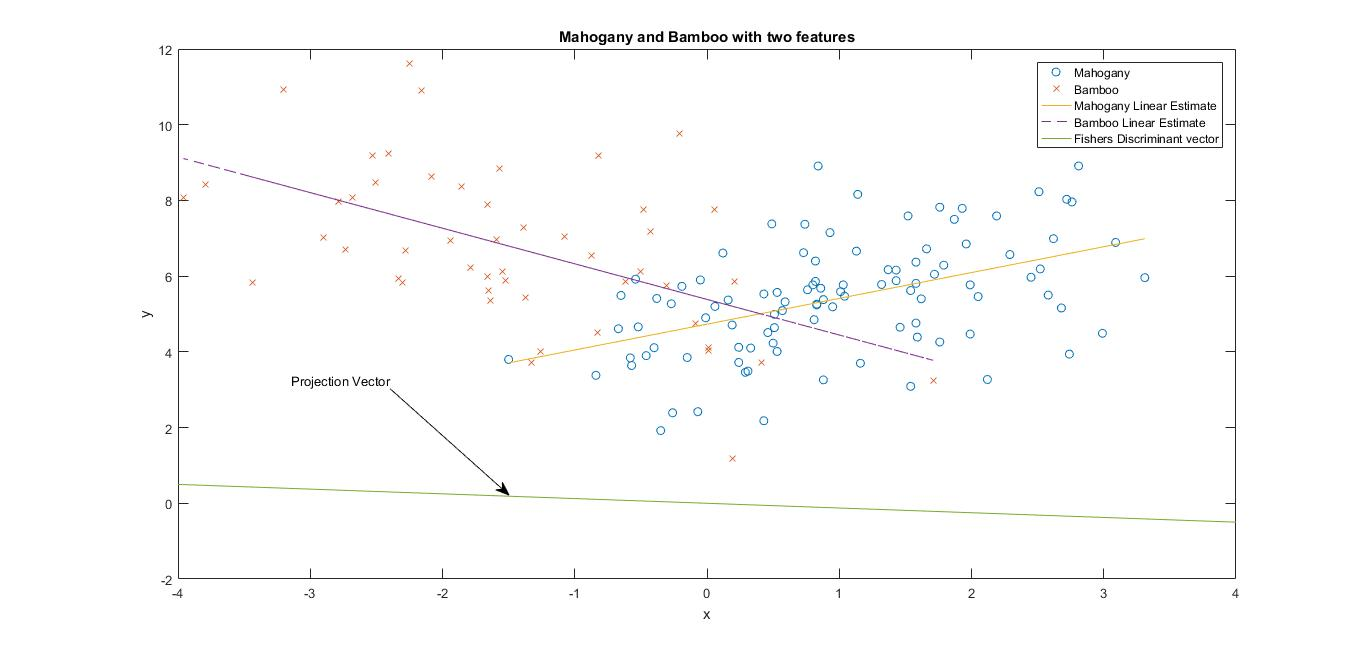
\includegraphics[scale=0.5]{q1_d}
   \caption{Mahogany and Bamboo with two features including the projection vector}\label{fig:q1_d}
\end{figure}
\clearpage
\newpage
\subsection*{(e)}
\begin{figure}[h]
  \hspace*{-6cm}
   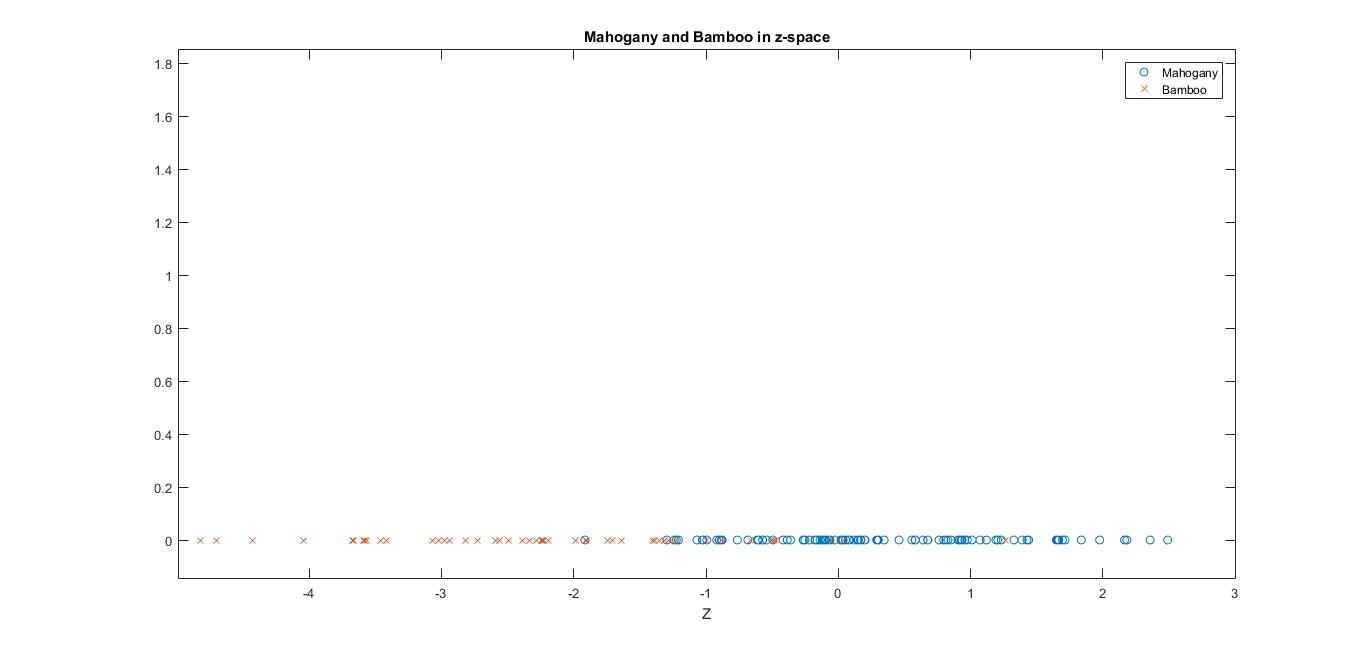
\includegraphics[scale=0.5]{q1_e}
   \caption{Mahogany and Bamboo projected to z space}\label{fig:q1_e}
\end{figure}
$$P[M] = \frac{\#Number of Mahogany In Sample in z-space}{\#Total Sample Size in z-space} = \frac{100}{150}=\frac{2}{3}$$
$$P[B] = \frac{\#Number of Bamboo In Sample in z-space}{\#Total Sample Size in z-space} = \frac{50}{150}=\frac{1}{3}$$
$$m_{M} =\frac{1}{M} \sum_{z}^{}M_z = 0.3191$$
$$m_{B} =\frac{1}{B} \sum_{z}^{}B_z = -2.251$$
$$\sigma_{M} = 0.9383$$
$$\sigma_{B} = 1.3001$$
Using only the prior prob. we can come up with a simple classifier that will be correct 66\% of the time. We say it is a Mahogany every time since prior Prob. of Mahogany $2*$ prior Prob. of Bamboo . 
\subsection*{(g) Verify}
 \[
 a^T\mu_M =
   \begin{bmatrix}
    0.9705&-0.1211
  \end{bmatrix}
  *
  \begin{bmatrix}
   1.0044\\
   5.4160
  \end{bmatrix}
 =0.3191= \mu_M
\]
 \[
 a^TK_Ma =
   \begin{bmatrix}
    0.9705&-0.1211
  \end{bmatrix}
  *
  \begin{bmatrix}
    1.0852 & 0.7399\\
    0.7399 & 2.1879
  \end{bmatrix}
  *
   \begin{bmatrix}
    0.9705\\
    -0.1211
  \end{bmatrix}
 =0.8804= \sigma_{M}^2
\]
 \[
 a^T\mu_B =
   \begin{bmatrix}
    0.9705&-0.1211
  \end{bmatrix}
  *
  \begin{bmatrix}
   -1.4752\\
    6.7724
  \end{bmatrix}
 =-2.2517= \mu_B
\]
 \[
 a^TK_Ba =
   \begin{bmatrix}
    0.9705&-0.1211
  \end{bmatrix}
  *
  \begin{bmatrix}
    1.3980 &  -1.3145\\
   -1.3145 &  4.4088
  \end{bmatrix}
  *
   \begin{bmatrix}
    0.9705\\
    -0.1211
  \end{bmatrix}
 =1.6904= \sigma_{B}^2
\]
\clearpage
\newpage
\subsection*{(h)}
\begin{figure}[h]
  \hspace*{-6cm}
   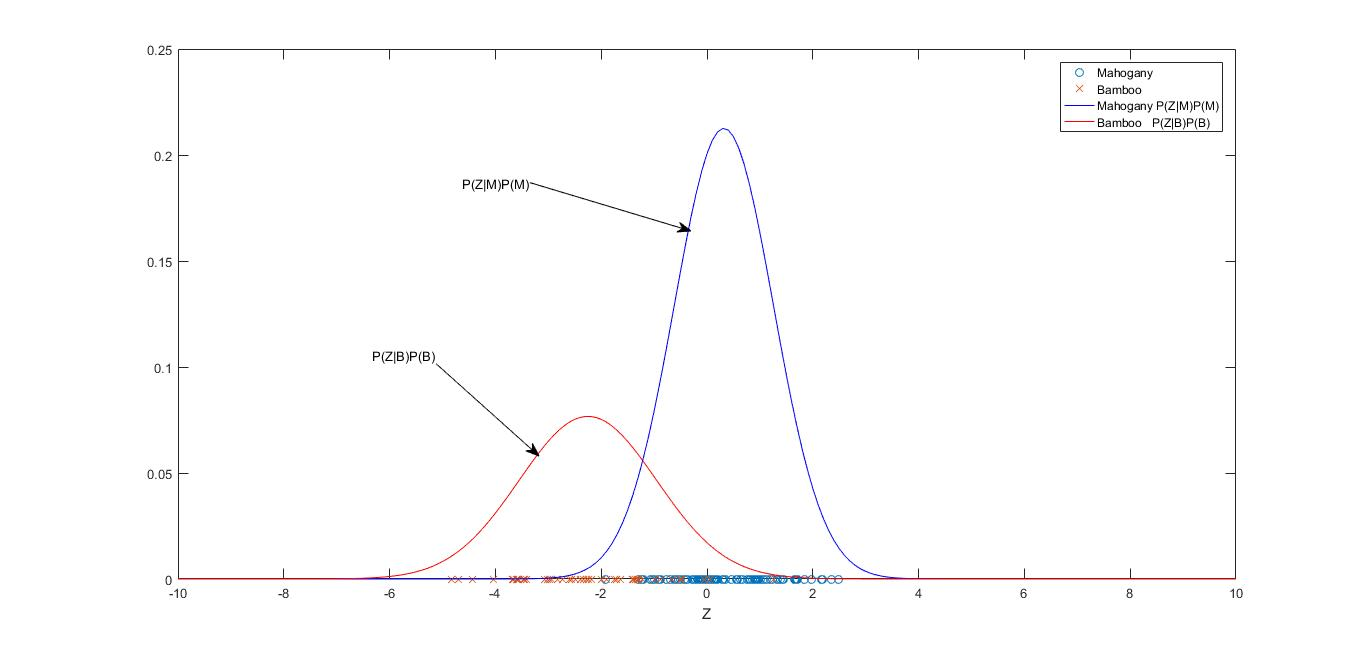
\includegraphics[scale=0.5]{q1_g_1}
   \caption{$P[z\vert M]P[M]$ and $P[z\vert B]P[B]$}\label{fig:q1_g_1}
\end{figure}
\clearpage
\newpage
\subsection*{(i)}
By solving the quadratic equation we get the following two decision boundary values\\
$MAP_1 = -1.0656$ and $MAP_2 = 7.2927$\\\\
So anything between $MAP_1$ and $MAP_2$ is going to be labeled as Mahogany and anything out side of this region is going to be labeled as Bamboo
\begin{figure}[h]
  \hspace*{-6cm}
   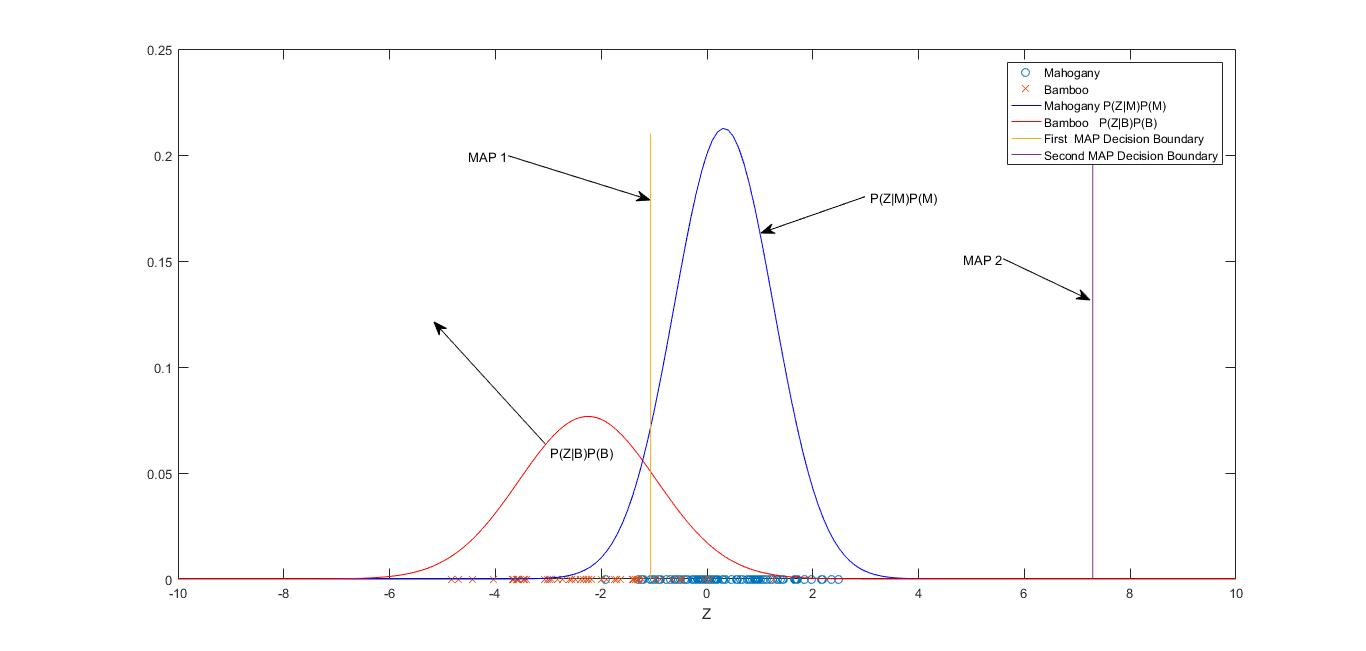
\includegraphics[scale=0.5]{q1_g}
   \caption{$P[z\vert M]P[M]$ and $P[z\vert B]P[B]$ with MAP decision boundaries }\label{fig:q1_g}
\end{figure}
\clearpage
\newpage
\subsection*{(j) Confusion matrix}
Using the MAP decision bounderies above we get Table \ref{tab:1} \\
\begin{table}
	\centering
	\hspace*{-1cm}
	\begin{tabular}{ |c|c|c|c|c|c|c|} 
	\hline
	&B &M\\
	\hline
	 B&0.2733&0.06\\
	\hline
           M&0.06&0.6267\\
           \hline
	\end{tabular}
	\caption{Confusion Matrix for the data} \label{tab:1}
\end{table}•\\
From this we get error rate of \\
$$error rate  = P[B,M]+P[M,B] = 0.1$$
Using the MAP decision bounderies above we get Table \ref{tab:2}(using Q functions refer to code) \\
\begin{table}
	\centering
	\hspace*{-1cm}
	\begin{tabular}{ |c|c|c|c|c|c|c|} 
	\hline
	&B &M\\
	\hline

	 B&0.2731&0.0603\\
	\hline
           M&0.0603&0.62\\
           \hline
	\end{tabular}
	\caption{Confusion Matrix for Normal approximation} \label{tab:2}
\end{table}•\\\\
From this we get error rate of \\
$$error rate  = P[B,M]+P[M,B] = 0.1206$$

\clearpage
\newpage

\begin{appendix}
\section*{Code Appendix}
\lstinputlisting[language=Octave]{hm8.m} 
\end{appendix}•
\end{document}